%%%%%%%%%%%%%%%%%%%%%%%%%%%%% -*- Mode: Latex -*- %%%%%%%%%%%%%%%%%%%%%%%%%%%%
%% 04-14-intro.tex -- Priority Ranked Software Inspection
%% Author          : Aaron A. Kagawa
%% Created On      : Mon Sep 23 11:52:28 2004
%% Last Modified By: Aaron Kagawa
%% Last Modified On: Sat Feb  5 13:25:36 2005
%% RCS: $Id$
%%%%%%%%%%%%%%%%%%%%%%%%%%%%%%%%%%%%%%%%%%%%%%%%%%%%%%%%%%%%%%%%%%%%%%%%%%%%%%
%%   Copyright (C) 2004 Aaron A. Kagawa
%%%%%%%%%%%%%%%%%%%%%%%%%%%%%%%%%%%%%%%%%%%%%%%%%%%%%%%%%%%%%%%%%%%%%%%%%%%%%%%


\chapter{Introduction}
Software inspection is defined as: ``A formal evaluation technique in which
software requirements, design, or code are examined in detail by a person
or group other than the author to detect faults, violations of development
standards, and other problems...'' \cite{Gilb93}. Software inspection, or
software review as it is sometimes called, can have fantastic results:
``Rigorous inspection can remove up to 90 percent of errors from a software
product before the fist test case is run'' \cite{Glass03, Bush90}.

Since Michael Fagan invented the inspection technique in 1976, there have
been many variations on the general concept of inspection. We now have
Fagan Inspection \cite{Fagan76}, Software Inspection \cite{Gilb93},
High-Impact Inspection, Phased Inspection, ``regular'' software inspection,
software reviews, code walkthroughs, inspections without meetings, and many
more different twists on the original concept.  Each of these techniques
claim to be the best inspection method for their certain circumstances. For
example, some argue that the inspection meeting is a waste of time and
resources \cite{Johnson97, Johnson98, Votta93}. Others argue that the
inspection meeting is critical for supporting social and educational
aspects of inspection \cite{Johnson98}.

My research is different from traditional inspection research. Instead of
asking how to conduct the inspection process, I ask how to determine what
to inspect, when to conduct inspections, and more importantly if inspection
is really needed for a particular piece of code. In this proposal, I will
describe how the selection of a document for inspection can create problems
for organizations with limited inspection resources. I will then propose a
new inspection document selection technique called Priority Ranked
Inspection and evaluate its effectiveness.


%%Since the introduction of inspections by Michael Fagan, there have been
%%numerous views, descriptions, and process that have been proposed by
%%various authors and researchers. Some of these include; Fagan Inspections
%%\cite{Fagan76}, Software Inspections \cite{Gilb93}, High-Impact
%%Inspections, and Phased Inspections just to name a few. Throughout this
%%paper I will use the lower cased inspection to represent all inspection
%%techniques.

\section{The Problem of Limited Resources for Software Inspections}
The use of software inspection has reported outstanding results in
improving productivity and quality. One study has found that when the
inspection process is followed correctly, up to 95 percent of defects can
be removed before entering the testing phase \cite{Bush90}. In another
success story, the Jet Propulsion Laboratory (JPL) adopted inspection to
identify defects and experienced a savings of 7.5 million dollars by
conducting 300 inspections \cite{Bush90a}. This statistic is very
impressive. However, what is not emphasized is each inspection had an
average total cost of 28 hours. Using that average cost, the total cost for
JPL's inspection process was 8,400 hours or roughly 4 years of work.

The JPL experience illustrates a fundamental problem with inspections:
better results come from substantial investment \cite{Gilb93}. Not all
organizations have the time or the money to invest in full or complete
inspections. In most cases, organizations have limited funds or resources
that can be devoted to inspections. For example, a manager may only have
200 hours of a project schedule to allocate towards quality assurance
including inspections. Such organizations must decide how to best utilize
their limited inspection resources. This realistic management of
inspections directly contradicts the classical inspection adage of ``when a
document is ready, you should inspect it''. The bottom line is that most
organizations cannot inspect every document.

The traditional inspection process begins with the initiation phase, or
sometimes called the planning stage, in which authors volunteer their
documents for inspection \cite {Gilb93}. A inspection leader checks the
document against entry criteria to determine if the document is ready for
inspection \cite{Ebenau94, Gilb93}. Again this process works very well for
organizations, like JPL, that have the resources to inspect every document
after every significant change. However, I believe that this phase of
inspection is a major problem for organizations that do not have the
necessary resources, because the process does not consider that some
documents are ``better'' to inspect than others. A simple illustration of
this fact is that 80 percent of defects come from 20 percent of the system
\cite{Boehm01}.  Thus, volunteering a document from the defect-prone 20
percent will likely be ``more in need of inspection'' than any other part
of the system.

Furthermore, the current literature \cite{Ebenau94, Wiegers02, Gilb93} on
inspections does not provide specific insights into the trade-offs between
inspecting some documents and not inspecting others.  However, Tom Gilb and
Dorothy Graham provide two recommendations to use when inspection resources
are limited; sampling and emphasizing up-stream documents \cite{Gilb93}.
The use of sampling involves inspecting various areas of a system to
identify areas of interest. Up-stream documents are documents that define
high-level requirements or designs.  Inspecting up-stream documents ensures
that the requirements are correct before any implementation is started.
Although, these are very useful recommendations, they do not provide much
specific guidance of how best to use limited inspection resources.

%%For example, consider the following scenario:
%%\begin{quotation}
%%  \textit{The FooBar organization has enough resources available to conduct
%%    two inspections a week. However, this organization creates and finishes
%%    10 different documents each week. How do they select 2 documents from
%%    the possible 10 to inspect? To be fair to all developers they use a
%%    round-robin type approach by allowing a different developer to
%%    volunteer a document for inspection. This approach is fairly successful
%%    and at least they are conducting inspections. But, are they inspecting
%%    the right documents? Obviously, this organization is unavoidably
%%    letting 8 documents slip through the inspection-crack and could be
%%    releasing documents that have critical defects.}
%%\end{quotation}


\section{The Priority Ranked Inspection Approach}
To address some of the problems associated with conducting inspections with
limited resources, I propose a new inspection process called ``Priority
Ranked Inspection'', (PRI). The primary goal of PRI is to optimize the
selection of documents for inspection by distingushing what documents are
``more in need of inspection'' (MINI) versus documents that are ``less in
need of inspection'' (LINI). In addition, PRI will rank each document
according to this determination in hopes of prioritizing the documents that
need to be inspected. The converse is also true: PRI will identify
documents that might not need to be inspected.

As I have shown in the previous section, it is extremely difficult for
organizations with limited inspection resources to inspect every document
before it exits the development process. Therefore, unlike traditional
inspection process, PRI does not require that all documents be inspected.
Instead, PRI is intended to help these organizations in two ways. First,
PRI is intended to be able to identify documents in the current development
process that need to be inspected. This will allow organizations to make an
educated guess at what documents need to be inspected and what documents
can be skipped. Second, it is unavoidable that some documents with critical
defects will finish the development process without being inspected.
Therefore, PRI is also intended to identify documents for inspection
regardless if a document is currently in the development process or not.

%%In the same ways that Software Inspection \cite{Gilb93} is an inspection
%%process, Priority Ranked Inspection is also an inspection
%%process. However, the differences between the two inspection processes lie
%%in the recognition that not all organizations have the necessary resources 
%%to inspect everything. Therefore, PRI is tailored to the organizations with 
%%limited resources. 

There are four primary steps in the Priority Ranked Inspection (PRI)
process. The following list is short description of each of the steps. The
following sub-sections provide a summary description of each step.

\begin{enumerate}
\item The creation of the PRI weighting function, which distinguishes
  MINI documents from LINI documents. The weighting function design
  includes two steps: 
\begin{enumerate}
\item Selection of product and process measures to use in the PRI
  weighting function.
\item Creation of a numerical weighting system that assigns a weight for
  each measure and the calibration of this weighting system.
\end{enumerate}
\item The selection of a document for inspection based on the PRI
  ranking.
\item The actual inspection of the selected document.
\item Adjustment of product and process measure selection and
  calibration based on the results of the inspection.
\end{enumerate}


\subsection{Step 1a: Selection of Product and Process Measures}
The PRI weighting function which distinguishes MINI documents from LINI
documents will be generated automatically from various product and process
measures. Product measures are usually obtainable from direct analysis of
source code.  For example, lines of code, complexity, and number of
children are a few examples of product measures. On the other hand, process
measures are collected from the actual software development process. The
amount of developer 'effort' and the number of defects are examples of
process measures. One might ask, what specific measures should PRI
consider? The answer: it depends on the specific situation. Different
projects and organizations could have a different set of measures in
defining the optimum PRI weighting function and ranking. Therefore, a major
component of the PRI process is the selection of the measures.

Software quality measures are one example of the type of product and
process measures that could be used in PRI. Software inspection has two
primary goals; increase quality and productivity. For this research I am
primarily concerned with increasing quality. The successful inspection of a
document has two main results: finding defects which, once removed,
increases software quality or not finding defects thus indicating high
software quality. Software quality is vaguely defined as ``the degree to
which software possesses a desired combination of attributes''
\cite{IEEEGlossary83}. Some of the possible measures of quality include:
portability, reliability, efficiency, usability, testability,
understandability, and modifiability \cite{Glass03}. Some other widely
accepted measures of quality include defect density and complexity.
Whatever definition used for quality, inspections aim to increase or
validate the level of quality in software.  Therefore, the same measures of
software quality will also provide good indications of what documents need
inspection. For example, finding documents that have low portability,
reliability, efficiency, usability, testability, understandability, and
modifiability would provide a good indication that the documents are MINI.

Based on the previous example, the quality-specific product and process
measures can be extracted and used in the PRI weighting function. Table
\ref{table:step1a} is an example of the PRI ranking of a software project
that contains three documents.  Presented in the table are the measures and
values that are used in the PRI ranking. Due to constraints of the paper
size, the table presents only a couple of the measures discussed above.
However, any number of measures can be used in the PRI weighting function.

\begin{table}[htbp]
  \caption{Step 1a - Example PRI ranking - After Measure Selection}
  \label{table:step1a}
  \begin{center}
    \begin{tabular}{|l|l|l|l|l|l|l|} \hline
      {\bf Document} & {\bf PRI Ranking} & {\bf Reliability} & 
      {\bf Efficiency} & {\bf Testability} & {\bf ...} \\ \hline
Foo.java & MINI & 3 & 4 & 2 & ...  \\ \hline
Bar.java & LINI & 4 & 2 & 6 & ...  \\ \hline
Baz.java & LINI & 1 & 2 & 3 & ...  \\ \hline
    \end{tabular}
  \end{center}
\end{table}

Table \ref{table:step1a} is an illustration of a fictitious PRI ranking.
See Chapter \ref{chapter:system}: Hackystat PRI Extension for more details
about the exact calculations necessary to create a PRI weighting function
and ranking.


\subsection{Step 1b: Calibration of the Product and Process Measures}
Only selecting what measures to be used in the PRI weighting function is
not adequate, because some measures are more important than others. For
example, an organization may find that testability has a greater positive
impact on the PRI weighting function than efficiency. Therefore, Step 1b of
the PRI process is the calibration of the measures' importance. The
calibration of the measures is based on a numerical weighting system. Each
measure will be assigned a numerical weight and will be individually
calibrated. The numerical weighting system and the calibration creates a
PRI ranking, which provides a priority ranking of the documents.

Using the same example (Table \ref{table:step1a}) from the previous
section, imagine that the organization has found testability to be a
leading indicator in defect prevention. Therefore, the calibration is
adjusted and the values of testability are given a higher weight than the
other measures. This finding changes the PRI weighting function and
ranking. The following table (Table \ref{table:step1b}) shows the new PRI
ranking after the calibration.

\label{table:step1b_trial}
\begin{table}[htbp]
  \caption{Step 1b - Example PRI ranking - After Measure Calibration}
  \label{table:step1b}
  \begin{center}
    \begin{tabular}{|l|l|l|l|l|l|l|} \hline
      {\bf Document} & {\bf PRI Ranking} & {\bf Reliability} & 
      {\bf Efficiency} & {\bf Testability} & {\bf ...} \\ \hline
Bar.java & MINI & 4 & 2 & 6 & ...  \\ \hline
Foo.java & MINI & 3 & 4 & 2 & ...  \\ \hline
Baz.java & LINI & 1 & 2 & 3 & ...  \\ \hline
    \end{tabular}
  \end{center}
\end{table}

Notice that, as a result of the calibration, the PRI ranking for Bar.java
has changed from LINI to MINI. This illustrates that the PRI weighting
function and ranking can be flexible and that it has the pontential to
reflect different development processes within different organizations.


\subsection{Step 2: Selecting a Document for Inspection Based on the PRI
  Ranking} After the PRI weighting function and ranking is in place,
an organization may use PRI to select documents for inspection. To select a
document for inspection they simply consult the PRI ranking and find a MINI
document (a document deemed more in need of inspection). This ranking will
help constrain the number of possible documents that can be considered for
inspection.

For example, in the example presented in Table \ref{table:step1b}, an
organization should select Bar.java for the inspection, because it ranked
the highest of the three documents. During the next inspection meeting,
Foo.java should be inspected. However, Baz.java could be skipped, thus
saving inspection resources.

Using the PRI ranking to select documents for inspection has three primary
benefits. First, it can enhance the selection or the volunteering process
of a document for inspection. Second, it can identify documents for
inspection that a volunteering process typically does not. Third,
inspecting a MINI document will generate more critical defects than
inspecting a LINI document.


\subsection{Step 3: Conducting an Inspection of the Selected Document}
Once the document is selected, a traditional inspection process can begin.
PRI does not have any special processes for this step. An organization can
choose to use any traditional inspection process (i.e., Software
Inspection, Fagan Inspection, In-Process Inspection). In other words, the
PRI process is an outer layer that wraps around an already established
inspection process to enhance the selection of documents.  Therefore, in
this research I will not discuss or evaluate traditional inspection
concepts like; inspection leaders, preparation time, etc.


\subsection{Step 4: Adjustment of the Measure Selection and Calibration}
After the inspection of a document, the results can be used to further
improve the PRI weighting function and ranking. For example, if the PRI
weighting function appears to be incorrect, because it ranked a document as
MINI but no major defects were found, then the PRI weighting function
should be adjusted to classify this document as LINI. This adjustment can
be achieved in two ways. First, one could add more product and process
measures to make the PRI weighting function more robust. Alternatively, one
could calibrate the current measures to refine and correct the PRI
weighting function and ranking.  In either case, an incorrect PRI weighting
function will provide data to help make future PRI weighting functions
better. This process should be an ongoing evolving activity.

For example, consider the example presented with Foo.java, Bar.java, and
Baz.java. If an organization has found results that suggest that efficiency
is a leading indicator of defects, then it should be calibrated with a
higher weight.



\section{The Hackystat PRI Extension}
To successfully use PRI, the determination of MINI and LINI must be
obtainable for a very low cost. In other words, if the weighting function
takes three months to generate, a software project will have long past the
need for those specific recommendations. Therefore, this determination must
be obtained in real-time.

One way of obtaining weighting function values in real-time is through the
use of the Hackystat system. Hackystat is a framework for collecting and
analyzing software product and development process metrics in real-time.
For more information about the Hackystat system see Chapter
\ref{chapter:hackystat}.  For this proposed research, I have created an
extension to the Hackystat system called the Hackystat PRI Extension
(hackyPRI for short). hackyPRI provides a real-time PRI weighting function
and ranking. Figure \ref{fig:intro-WorkspacePRIAnalysis} demonstrates the
PRI weighting function and its ranking for a software project that is
obtainable from the Hackystat PRI Extension.

\begin{figure*}[ht]
  \centering
  \includegraphics[width=1.00\textwidth]{WorkspaceQuality.eps}
  \caption{The Workspace PRI analysis. Workspaces are listed with its
  respective PRI ranking and measures.}
  \label{fig:intro-WorkspacePRIAnalysis}
\end{figure*}

The Hackystat PRI Extension will be implemented to fully support all 4
steps of the PRI process. The next subsections demonstrate how hackyPRI
supports each of the 4 steps. It is important to note that PRI is a
proposed \textit{process}, therefore many different tools can support it.
Using the Hackystat PRI Extension is not required to conduct PRI
inspections.



\subsection{Step 1a: Selection of Product and Process Measures}
The Hackystat system provides a standard set of product and process
measures, these measures are called Sensor Data Types within the Hacksytat
system, and the means of its collection. Initially, I have developed
hackyPRI to use all of the measures obtainable from Hackystat. In addition,
I have begun to implement a several new Hackystat Sensor Data Types
(measures), that I feel will aid the PRI weighting function.

Each column in Figure \ref{fig:intro-WorkspacePRIAnalysis} is a measure
that is obtainable from Hackystat. Each measure will be automatically and
unobtrusively collected by Hackystat and directly fed in to the hackyPRI
extension.


\subsection{Step 1b: Calibration of Product and Process Measures}
Each measure and its numerical weight will be stored within the hackyPRI
extension. The numerical weights are not shown in Figure
\ref{fig:intro-WorkspacePRIAnalysis}. However, the calibration and
weighting system works behind the scenes to rank each document. For
example, the coverage measure is assigned a numerical weight of 3 if the
coverage value equals 100 percent, 2 if the coverage value is below 90
percent, 1 if the coverage value is below 80 percent, and 0 if the coverage
value is below 70 percent. See Chapter \ref{chapter:system} for a detailed
description about the numerical weighting system.


\subsection{Step 2: Selecting a Document for Inspection Based on the PRI
  Ranking} Using the PRI Hackystat analysis, an organization should
select a document at the bottom of the PRI ranking table for inspection.
The higher the document is in the table, the more it is likely to be LINI.


\subsection{Step 3: Conducting an Inspection of the Selected Document}
Once a document is selected it can be inspected. One interesting side
effect of the PRI ranking is that specific statistics and measures
can be presented during the inspection process. For example, if a document
is selected because it has low coverage, then the inspection can focus on
why the coverage is low.

\subsection{Step 4: Adjustment of the Measure Selection and Calibration}
If a document is shown to be incorrectly ranked, then an adjustment of the
PRI weighting function is necessary. This can be accomplished by adding
more Hackystat measures to the PRI weighting function or recalibrating the
numerical weights associated with the measures. See Chapter
\ref{chapter:system} for a detailed description of the calibration process
for the hackyPRI extension.



\section{Thesis Statement}
The thesis statement of this research is as follows; Priority Ranked
Inspection can distinguish documents that are more in need of inspection
(MINI) from others that need inspection less (LINI). This thesis statement
can be decomposed into the following three main claims, which are based on
the intended benefits of PRI.

\begin{enumerate}
\item PRI can enhance the volunteer-based document selection process.
\item PRI can identify documents that need to be inspected that are not
  typically identified by volunteering.
\item Documents that are deemed more in need of inspection (MINI) will
  generate more critical defects than documents deemed less in need of
  inspection (LINI).
\end{enumerate}

My first claim states that PRI can enhance the selection process. In the
traditional inspection process, this selection process is based on a
developer selecting and volunteering a document for inspection.  This claim
is an intended benefit of PRI because in the traditional inspection process
the number of documents that a developer must select from can vary widely.
If PRI can provide the MINI documents, then the developer can focus his
selection on a smaller set of documents.

My second claim states that PRI can identify documents that have slipped
through the cracks in the development process. For an organization with
limited inspection resources it is not possible to inspect every document.
Therefore, it is inevitable that some documents that need to be inspected
have not been.

My third and last claim states that the inspection of MINI documents will
generate more critical defects than LINI documents. This claim is very
important to the PRI process because if this claim is proven to be false,
then the PRI process cannot solve the limited inspection resource problem.



\section{Evaluation}
This section provides a short description of the methodologies used to
evaluate my thesis claims. Chapter \ref{chapter:evaluation}, Evaluation
Methodology provides a detailed explanation of the methodologies and
procedures that will be used in the evaluation of PRI.

I will evaluate the main thesis of this proposed research by testing each
of my three claims. In this evaluation, I will be studying the inspection
process of the Hackystat system developed by the Collaborative Software
Development Laboratory. I will also be using the developers of Hackystat as
subjects in my evaluation.

My first claim states that PRI enhances the volunteer-based document
selection process. To evaluate this claim, I will conduct a qualitative and
quantitative evaluation.  First, I will assess the developers' current
selection process by asking them to rank a few documents based on what
documents they think are more in need of inspection. Then I will provide
them with the PRI ranking of those same documents and ask them which
rankings would they change. After this qualitative evaluation, I will ask
CSDL to inspect a few documents to evaluate the validity of the developers'
subjective ranking and the PRI ranking.

My second claim states that PRI can identify MINI documents that are not
typically identified by the volunteering process. To evaluate this claim, I
will ask CSDL to inspect a few documents that have not been identified in
the previous evaluation.

My third and last claim states that the inspection of MINI documents will
generate more critical defects than LINI documents. Throughout the
previous two studies I will have collected information about approximately
20 inspections. By quantitatively analyzing the results of these
inspections I will be able to provide supporting evidence for this claim.


\section{Structure of the Proposal}
The remainder of this proposed research is as follows. Chapter
\ref{chapter:relatedwork} discusses previous studies that influenced this
research. Chapter \ref{chapter:hackystat} and Chapter \ref{chapter:system}
contains a detailed description of the Hackystat system and the Priority
Ranked Inspection (PRI) Hackystat extension. Chapter
\ref{chapter:evaluation} discusses the evaluation methodology that will be
implemented to evaluate the claims and benefits of PRI. Chapter
\ref{chapter:contribution} discusses the contributions and future
directions of this research. Finally, Chapter \ref{chapter:timeline}
provides a detailed timeline of this proposed research.














% LocalWords:  Kagawa Sep
